\chapter{Wybrany algorytm przetwarzania danych i techniki optymalizacji programów komputerowych}
\section{Opis i analiza Szybkiej Transformaty Fouriera}
\subsection{Podstawy matematyczne algorytmu FFT}
\textbf{Przekształcenie Fouriera} (ang. \textit{Fourier Transform}) dla sygnałów ciągłych służy do wyznaczania widma częstotliwościowego $X(j\omega)$ sygnału czasu ciągłego $x(t)$ \cite{ZielinskiDSP}. Wzory przekształcenia prostego i odwrotnego definiuje się następująco \cite{ZielinskiDSP}:

\begin{equation}
X(j\omega) = \int_{-\infty}^{\infty} x(t)\, e^{-j\omega t}\, dt,
\qquad
x(t) = \frac{1}{2\pi}\int_{-\infty}^{\infty} X(j\omega)\, e^{j\omega t}\, d\omega
\end{equation}

gdzie $\omega = 2\pi f$ oznacza pulsację, a $f$ częstotliwość wyrażoną w hercach.

Aby całka określająca $X(j\omega)$ była zbieżna, sygnał $x(t)$ musi spełniać tzw. \textbf{warunki Dirichleta}: być bezwzględnie całkowalny, mieć skończoną liczbę ekstremów oraz skończoną liczbę punktów nieciągłości w dowolnym skończonym przedziale \cite{ZielinskiDSP}.

Matematyczne podstawy ciągłej transformaty Fouriera są jednak nie do końca przydatne w świecie cyfrowego przetwarzania sygnałów, właśnie z uwagi na fakt, że sygnały, na których pracują maszyny cyfrowe, są dyskretne, a nie ciągłe. W tym celu definiuje się dyskretną transformatę Fouriera, która powstaje w wyniku dyskretyzacji szeregu Fouriera dla sygnału okresowego o okresie $N$ \cite{ZielinskiDSP}.

W systemach cyfrowych przetwarzany sygnał dostępny jest w postaci skończonego ciągu próbek $x(n)$, $n = 0, 1, \dots, N-1$, pobranych z częstotliwością próbkowania $f_{pr}$. Powyższy wzór na ciągłą transformatę Fouriera nie da się więc bezpośrednio zastosować. Zamiast niego widmo sygnału wyznacza się za pomocą \textbf{dyskretnej transformacji Fouriera} (DFT, ang. \textit{Discrete Fourier Transform}). Matematyczne przekształcenia dla prostej i odwrotnej DFT definiuje się następująco \cite{ZielinskiDSP}:

\begin{equation}
X(k) = \frac{1}{N}\sum_{n=0}^{N-1} x(n)\, e^{-j\frac{2\pi}{N}kn},
\qquad k = 0, 1, \dots, N-1
\label{eq:dft_analiza}
\end{equation}

\begin{equation}
x(n) = \sum_{k=0}^{N-1} X(k)\, e^{j\frac{2\pi}{N}kn},
\qquad n = 0, 1, \dots, N-1
\end{equation}

gdzie $k$ oznacza numer składowej widma, dla której wyliczana jest aktualnie wartość transformaty. Kolejnym składowym odpowiada pulsacja $\Omega_k = 2\pi k/N$.

Wygodnym uproszczeniem powyższych zapisów jest wprowadzenie tzw. \textbf{czynnika obrotu} (ang. \textit{twiddle factor})\cite{CormenIntroductionAlgorithms}:

\begin{equation}
W_N = e^{-j\frac{2\pi}{N}}
\label{eq:twiddle}
\end{equation}

co pozwala przedstawić parę wzorów DFT w zwartej postaci \cite{ZielinskiDSP}:

\begin{equation}
X(k) = \frac{1}{N}\sum_{n=0}^{N-1} x(n)\, W_N^{kn},
\qquad k = 0, 1, \dots, N-1
\label{eq:dft_analiza_wn}
\end{equation}

\begin{equation}
x(n) = \sum_{k=0}^{N-1} X(k)\, W_N^{-kn},
\qquad n = 0, 1, \dots, N-1
\label{eq:dft_synteza_wn}
\end{equation}


W inżynierii oprogramowania do porównywania wydajności algorytmów powszechnie wykorzystuje się \textbf{notację dużego O} (ang. \textit{Big O notation}), opisującą tempo wzrostu liczby wykonywanych operacji wraz ze długości wektora przetwarzanych danych wejściowych $N$. Zapis $O(g(N))$ oznacza, że liczba wykonywanych operacji rośnie nie szybciej niż funkcja $g(N)$ pomnożona przez pewną stałą, dla odpowiednio dużych $N$ \cite{CormenIntroductionAlgorithms}.

Innymi słowy, notacja ta pomija czynniki stałe i wyrazy niższego rzędu, skupiając się na tym, jak rośnie liczba operacji wraz ze wzrostem rozmiaru danych wejściowych \cite{CormenIntroductionAlgorithms}.

Dla przykładu, bezpośrednie obliczenie wzoru \eqref{eq:dft_analiza} dla każdego z $N$ prążków widma wymaga $N$ mnożeń zespolonych, co dla całego wektora $X(k)$ wymaga wykonania zasadniczo $N^2$ mnożeń. W takim wypadku złożoność algorytmu DFT można określić jako $O(N^2)$. Przy ciągłym przetwarzaniu długich sygnałów złożoność ta stanowi istotne ograniczenie praktyczne. Jej redukcja jest możliwa dzięki zastosowaniu \textbf{algorytmu szybkiej transformacji Fouriera} (FFT, ang. \textit{Fast Fourier Transform}), który pozwala znacznie obniżyć koszt obliczeniowy.
\subsection{Szybka transformata Fouriera}
Redukcja złożoności obliczeniowej DFT jest możliwa dzięki zastosowaniu algorytmów określanych mianem szybkich transformacji Fouriera (FFT). Można w tym wypadku mówić o pewnym zbiorze rozwiązań, bazujących na tym samym koncepcie. Po raz pierwszy algorytm ten zaproponowano w latach sześćdziesiątych XX wieku w pracy \cite{CooleyTurkeyFFT}. Rodzina algorytmów FFT pozwala na znaczące obniżenie złożoności obliczeniowej, przy zachowaniu takiej samej poprawności obliczeń jak w przypadku klasycznego algorytmu DFT. FFT jest więc wydajnym sposobem na obliczenie DFT — jego złożoność obliczeniowa spada do rzędu $O(N\log_2 N)$ \cite{ZielinskiDSP}.

W pracy Cooleya-Tukeya \cite{CooleyTurkeyFFT} zaproponowano nowe podejście do obliczania dyskretnej transformaty Fouriera, polegające na rozłożeniu długiego sygnału, o $N$ próbkach, na kilka mniejszych grup. Następnie policzono transformatę osobno dla każdej z nich, by w ostatnim kroku połączyć wyniki w widmo całego sygnału.

Autorzy zauważyli również, że wybór $N$ będącego potęgą liczby 2 lub 4 jest szczególnie wygodny dla komputerów działających na liczbach binarnych. Co więcej, cały algorytm można było wykonać na tej samej tablicy danych, bez potrzeby rezerwowania dodatkowej pamięci na wyniki pośrednie \cite{CooleyTurkeyFFT}.

Zaproponowana metoda stała się inspiracją dla tworzenia kolejnych wariantów szybkiej transformaty Fouriera \cite{ZielinskiDSP}:

\begin{itemize}
    \item \textbf{Radix-2},
    \item \textbf{radix-4},
    \item \textbf{split-radix},
    \item \textbf{algorytm Gooda-Thomasa},
    \item \textbf{transformacja świergotowa (ang. \textit{chirp-Z})}.
\end{itemize}
Wszystkie realizują to samo przekształcenie, czyli dyskretną transformatę Fouriera, różnią się natomiast wewnętrznymi mechanizmami, takimi jak podejście do podziału danych czy długości pojedynczego bloku przetwarzanego sygnału \cite{ZielinskiDSP}.
Szczegółowy opis wariantów wykorzystanych w niniejszej pracy, wraz z ich implementacjami, przedstawiono w \cref{section:WariantyFFTUzyteWPracy}.

Do dalszej analizy teoretycznej posłuży popularny wariant FFT oparty na \textbf{podstawie 2} (ang. \textit{radix-2}), czyli podziale na dwa podzbiory, jako najprostszy do intuicyjnego wyjaśnienia.
Na algorytm w tej postaci składa się kilka podstawowych zagadnień, omówionych kolejno w dalszej części podrozdziału: sposób podziału danych, uporządkowanie próbek przed rozpoczęciem obliczeń oraz elementarna operacja arytmetyczna, powtarzana na każdym etapie.

Podział wektora wejściowego może być przeprowadzony na dwa podstawowe sposoby. W wariancie z \textbf{decymacją w czasie} (DIT, ang. \textit{Decimation in Time}) dzieli się próbki sygnału wejściowego na te o indeksach parzystych i nieparzystych, wykonuje DFT osobno na każdym zbiorze, a następnie odtwarza widmo całego sygnału z widm cząstkowych \cite{ZielinskiDSP}. W wariancie z \textbf{decymacją w częstotliwości} (DIF, ang. \textit{Decimation in Frequency}) postępuje się odwrotnie — dzieli się nie próbki wejściowe, lecz prążki widma wyjściowego \cite{ZielinskiDSP}.

Konsekwencją podziału jest to, że dane trafiają do obliczeń w innej kolejności niż ta pierwotna w sygnale wejściowym, więc na którymś etapie algorytmu należy je uporządkować. W algorytmach DIT robi się to na wejściu, przed właściwymi obliczeniami, i wynik otrzymuje się w kolejności naturalnej \cite{NumericalRecipesC}. W DIF jest odwrotnie — poprzestawiany jest dopiero wynik, na co zwrócono uwagę już w oryginalnej pracy \cite{CooleyTurkeyFFT}.

Samo przestawianie można wykonać na kilka różnych sposobów, z czego podstawowy polega na wielokrotnym dzieleniu próbek na parzyste i nieparzyste. Jest to jednak rozwiązanie nieefektywne, ponieważ dane sortowane są wielokrotnie \cite{ZielinskiDSP}. Okazuje się, że docelową pozycję każdej próbki da się wyznaczyć z użyciem operacji \textbf{permutacji bitowo-odwróconej} (ang. \textit{bit-reversal permutation}) \cite{CormenIntroductionAlgorithms}. Metoda ta ustawia w odwrotnej kolejności bity indeksu próbki wektora wejściowego \cite{ZielinskiDSP}, co pozwala dość niskim kosztem obliczeniowym poukładać wektor wejściowy w kolejności wymaganej przez algorytm DIT. Warto dodać, że wiele procesorów sygnałowych udostępnia sprzętowy mechanizm adresowania z odwróceniem bitów, co dodatkowo przyspiesza ten etap \cite{ZielinskiDSP}.

% ===== CLAUDE GENERATED START =====
Wynik tej operacji dla sygnału o długości $N = 16$ zestawiono w \cref{tab:bit_reversal} \cite{ZielinskiDSP}. Warto zauważyć, że w celu ponownego ustawienia próbek w pierwotnej kolejności wystarczy raz jeszcze wykonać tę samą operacje. W prezentowanej tabeli jako $n$ oznaczono indeks początkowy, a jako  $n'$ indeks po operacji bit-reversal.
\begin{table}[ht]
    \centering
    \caption{Permutacja bitowo-odwrócona indeksów próbek dla $N = 16$}
    \label{tab:bit_reversal}
    \begin{tabular}{@{}rccr@{\hspace{2.5em}}rccr@{}}
        \toprule
        $n$ & zapis dwójkowy & bity odwrócone & $n'$ &
        $n$ & zapis dwójkowy & bity odwrócone & $n'$ \\
        \midrule
        0 & \texttt{0000} & \texttt{0000} & 0  &  8  & \texttt{1000} & \texttt{0001} & 1  \\
        1 & \texttt{0001} & \texttt{1000} & 8  &  9  & \texttt{1001} & \texttt{1001} & 9  \\
        2 & \texttt{0010} & \texttt{0100} & 4  &  10 & \texttt{1010} & \texttt{0101} & 5  \\
        3 & \texttt{0011} & \texttt{1100} & 12 &  11 & \texttt{1011} & \texttt{1101} & 13 \\
        4 & \texttt{0100} & \texttt{0010} & 2  &  12 & \texttt{1100} & \texttt{0011} & 3  \\
        5 & \texttt{0101} & \texttt{1010} & 10 &  13 & \texttt{1101} & \texttt{1011} & 11 \\
        6 & \texttt{0110} & \texttt{0110} & 6  &  14 & \texttt{1110} & \texttt{0111} & 7  \\
        7 & \texttt{0111} & \texttt{1110} & 14 &  15 & \texttt{1111} & \texttt{1111} & 15 \\
        \bottomrule
    \end{tabular}
\end{table}
% ===== CLAUDE GENERATED STOP =====

Niezależnie od przyjętego wariantu uporządkowania danych, kolejną elementarną operacją wykonywaną na każdym etapie algorytmu FFT, bazujących na założeniach zaprezentowanych w \cite{CooleyTurkeyFFT}, jest tak zwana \textbf{operacja motylkowa} (ang. \textit{butterfly}) \cite{ZielinskiDSP}. Operacja ta pobiera parę liczb zespolonych $x(p)$ oraz $x(q)$, mnoży drugą z nich przez odpowiedni czynnik obrotu \eqref{eq:twiddle}, a następnie wyznacza sumę i różnicę otrzymanych w ten sposób wartości \cite{CormenIntroductionAlgorithms}:

\begin{equation}
x'(p) = x(p) + W_N^{k}\,x(q),
\qquad
x'(q) = x(p) - W_N^{k}\,x(q)
\label{eq:motylek}
\end{equation}

gdzie $p$ i $q$ oznaczają pozycje dwóch przetwarzanych elementów w tablicy danych, oddalone od siebie o połowę długości bieżącego etapu, a wykładnik $k$ — numer operacji motylkowej w obrębie tego etapu.

Istotną cechą tak zapisanej operacji jest to, że obie wartości wynikowe mogą zostać zapisane w tych samych komórkach pamięci, z których pobrano argumenty. Dzięki temu cały algorytm można zrealizować bez rezerwowania dodatkowej tablicy na wyniki pośrednie, co pozwala na zaoszczędzenie zasobów sprzętowych \cite{CooleyTurkeyFFT}. Graficzną reprezentację przepływu sygnałów w operacji motylkowej przedstawiono na \cref{fig:motylek-radix2}.

\begin{figure}[ht]
    \centering
    \definecolor{userblue}{RGB}{225, 243, 254}
    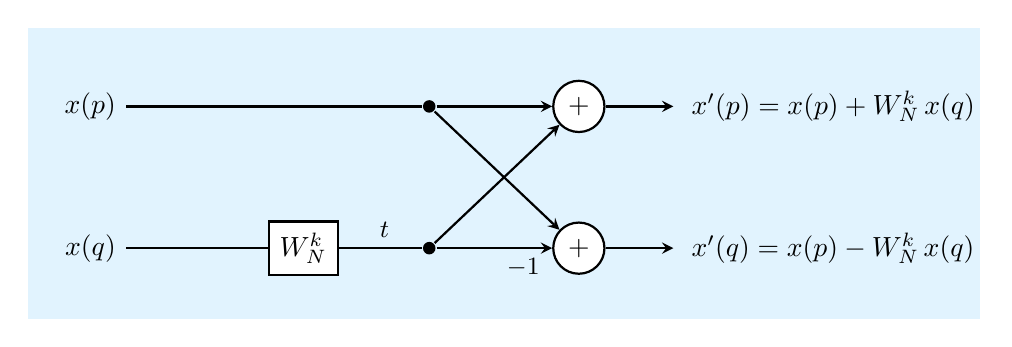
\begin{tikzpicture}[>=stealth, thick, scale=1, every node/.style={transform shape},
        sum/.style={circle, draw, thick, fill=white, inner sep=0pt, minimum size=6.5mm},
        dot/.style={circle, fill, inner sep=1.6pt}]

    \fill[userblue] (-1.5,-0.9) rectangle (10.6,2.8);

    % --- węzły wejściowe ---
    \node[anchor=east] (xp) at (-0.25,1.8) {$x(p)$};
    \node[anchor=east] (xq) at (-0.25,0)   {$x(q)$};

    % --- element mnożący przez czynnik obrotu ---
    \node[draw, thick, fill=white, inner sep=4pt] (w) at (2.0,0) {$W_N^{k}$};

    % --- punkty rozgałęzień ---
    \node[dot] (s) at (3.6,1.8) {};
    \node[dot] (t) at (3.6,0)   {};

    % --- sumatory ---
    \node[sum] (sp) at (5.5,1.8) {$+$};
    \node[sum] (sq) at (5.5,0)   {$+$};

    % --- gałąź górna ---
    \draw (xp.east) -- (s);
    \draw[->] (s) -- (sp);
    \draw[->] (s) -- (sq);

    % --- gałąź dolna ---
    \draw (xq.east) -- (w);
    \draw (w) -- node[above, font=\small, pos=0.55] {$t$} (t);
    \draw[->] (t) -- (sp);
    \draw[->] (t) -- node[below, font=\small, pos=0.75] {$-1$} (sq);

    % --- wyjścia ---
    \draw[->] (sp) -- (6.7,1.8);
    \draw[->] (sq) -- (6.7,0);
    \node[anchor=west] at (6.8,1.8) {$x'(p) = x(p) + W_N^{k}\,x(q)$};
    \node[anchor=west] at (6.8,0)   {$x'(q) = x(p) - W_N^{k}\,x(q)$};

    \end{tikzpicture}
    \caption[Operacja motylkowa algorytmu FFT o podstawie 2]{Operacja motylkowa (ang. \textit{butterfly}) algorytmu FFT o podstawie~2, opracowanie własne na podstawie \cite{ZielinskiDSP}}
    \label{fig:motylek-radix2}
\end{figure}

Zależności pomiędzy kolejnymi etapami algorytmu wygodnie jest przedstawić w postaci grafu przepływu sygnałów. Na \cref{fig:graf-fft-8} zobrazowano pełny przebieg obliczeń dla sygnału o długości $N = 8$, a więc dla $\log_2 8 = 3$ etapów, z których każdy składa się z $N/2 = 4$ operacji motylkowych.

\begin{figure}[H]
    \centering
    \definecolor{userblue}{RGB}{225, 243, 254}
    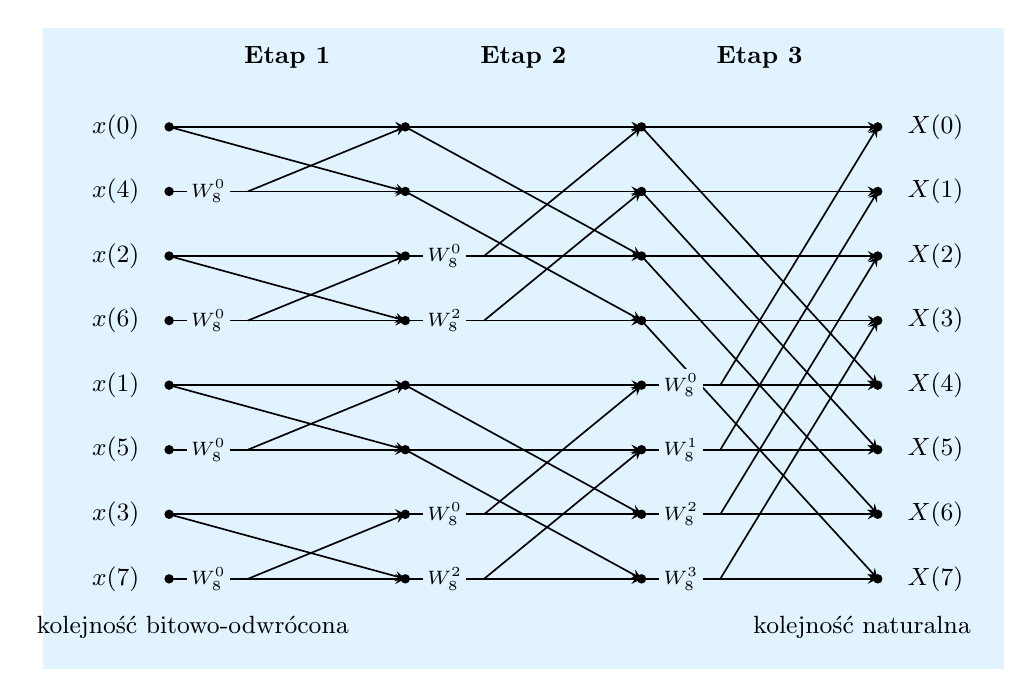
\begin{tikzpicture}[>=stealth, line width=0.6pt, scale=1, every node/.style={transform shape},
        tw/.style={fill=userblue, inner sep=1.6pt, font=\scriptsize}]

    \fill[userblue] (-1.6,-1.15) rectangle (10.6,7.0);

    % --- siatka węzłów: 4 kolumny (wejście + 3 etapy) x 8 wierszy ---
    \foreach \s in {0,1,2,3} {
        \foreach \r in {0,...,7} {
            \coordinate (n\s-\r) at ({\s*3.0}, {(7-\r)*0.82});
        }
    }

    % --- ETAP 1: pary wierszy (0,1), (2,3), (4,5), (6,7) ---
    \foreach \a/\b/\k in {0/1/0, 2/3/0, 4/5/0, 6/7/0} {
        \coordinate (m1-\b) at (1.0, {(7-\b)*0.82});
        \draw[->] (n0-\a) -- (n1-\a);
        \draw[->] (n0-\a) -- (n1-\b);
        \draw (n0-\b) -- (m1-\b);
        \draw[->] (m1-\b) -- (n1-\b);
        \draw[->] (m1-\b) -- (n1-\a);
    }

    % --- ETAP 2: pary wierszy (0,2), (1,3), (4,6), (5,7) ---
    \foreach \a/\b/\k in {0/2/0, 1/3/2, 4/6/0, 5/7/2} {
        \coordinate (m2-\b) at (4.0, {(7-\b)*0.82});
        \draw[->] (n1-\a) -- (n2-\a);
        \draw[->] (n1-\a) -- (n2-\b);
        \draw (n1-\b) -- (m2-\b);
        \draw[->] (m2-\b) -- (n2-\b);
        \draw[->] (m2-\b) -- (n2-\a);
    }

    % --- ETAP 3: pary wierszy (0,4), (1,5), (2,6), (3,7) ---
    \foreach \a/\b/\k in {0/4/0, 1/5/1, 2/6/2, 3/7/3} {
        \coordinate (m3-\b) at (7.0, {(7-\b)*0.82});
        \draw[->] (n2-\a) -- (n3-\a);
        \draw[->] (n2-\a) -- (n3-\b);
        \draw (n2-\b) -- (m3-\b);
        \draw[->] (m3-\b) -- (n3-\b);
        \draw[->] (m3-\b) -- (n3-\a);
    }

    % --- oznaczenia węzłów ---
    \foreach \s in {0,1,2,3} {
        \foreach \r in {0,...,7} {
            \fill (n\s-\r) circle (1.7pt);
        }
    }

    % --- czynniki obrotu (rysowane na końcu, aby nie były przesłaniane) ---
    \foreach \x/\r/\k in {%
        0.5/1/0, 0.5/3/0, 0.5/5/0, 0.5/7/0,
        3.5/2/0, 3.5/3/2, 3.5/6/0, 3.5/7/2,
        6.5/4/0, 6.5/5/1, 6.5/6/2, 6.5/7/3} {
        \node[tw] at ({\x}, {(7-\r)*0.82}) {$W_8^{\k}$};
    }

    % --- próbki wejściowe w kolejności bitowo-odwróconej ---
    \foreach \r/\idx in {0/0, 1/4, 2/2, 3/6, 4/1, 5/5, 6/3, 7/7} {
        \node[anchor=east, font=\small] at ({-0.25}, {(7-\r)*0.82}) {$x(\idx)$};
    }

    % --- prążki widma w kolejności naturalnej ---
    \foreach \r in {0,...,7} {
        \node[anchor=west, font=\small] at ({9.25}, {(7-\r)*0.82}) {$X(\r)$};
    }

    % --- opisy etapów i kolumn ---
    \node[anchor=south, font=\small\bfseries] at (1.5,6.35) {Etap 1};
    \node[anchor=south, font=\small\bfseries] at (4.5,6.35) {Etap 2};
    \node[anchor=south, font=\small\bfseries] at (7.5,6.35) {Etap 3};

    \node[anchor=north, font=\small] at (0.3,-0.35) {kolejność bitowo-odwrócona};
    \node[anchor=north, font=\small] at (8.8,-0.35) {kolejność naturalna};

    \end{tikzpicture}
    \caption[Graf przepływu sygnałów algorytmu FFT z decymacją w czasie dla $N = 8$]{Graf przepływu sygnałów algorytmu FFT o podstawie~2 z decymacją w czasie dla $N = 8$; każde skrzyżowanie linii odpowiada operacji motylkowej przedstawionej na \cref{fig:motylek-radix2}, opracowanie własne na podstawie \cite{ZielinskiDSP, NumericalRecipesC}}
    \label{fig:graf-fft-8}
\end{figure}

Graf ten dobrze ilustruje trzy własności algorytmu, istotne z punktu widzenia jego późniejszej implementacji. Po pierwsze, liczba etapów rośnie logarytmicznie wraz z długością przetwarzanego sygnału, a na każdym z nich wykonywanych jest $N/2$ operacji motylkowych, co daje łącznie $\frac{N}{2}\log_2 N$ mnożeń zespolonych i stanowi bezpośrednie źródło złożoności $O(N\log_2 N)$. Po drugie, próbki wejściowe podawane są w kolejności bitowo-odwróconej, dzięki czemu prążki widma otrzymuje się w kolejności naturalnej. Po trzecie, odległość w pamięci pomiędzy argumentami pojedynczej operacji motylkowej podwaja się z każdym kolejnym etapem — w pierwszym etapie łączone są próbki bezpośrednio sąsiadujące, natomiast w ostatnim oddalone od siebie o $N/2$ pozycji. Ta ostatnia cecha ma bezpośredni wpływ na skuteczność wykorzystania pamięci podręcznej procesora, co szerzej omówiono w \cref{section:TechnikiOptymalizacji}.

Operacja bit-reversal jest iteracyjnym sposobem na odpowiednie uporządkowanie tablicy wejściowej przed właściwym przetwarzaniem algorytmu FFT. Sam algorytm można jednak zapisać również z wykorzystaniem rekurencji. Oba warianty, zarówno iteracyjny jak i rekurencyjny są spotykane praktycznie \cite{NumericalRecipesC}. Rekurencja dobrze oddaje ideę podziału na coraz mniejsze podproblemy, natomiast w implementacjach nastawionych na wydajność (oraz w tych wykonywanych w systemach o ograniczonej pamięci) częściej stosuje się wariant iteracyjny, w którym wystarczy pętla po kolejnych etapach \cite{NumericalRecipesC}.

Przedstawione powyżej koncepcje stosowane w algorytmie FFT składają się łącznie na kompletny algorytm. Jego minimalną postać, w wariancie radix-2 z decymacją w czasie, przedstawiono na \cref{alg:fft-dit-iteracyjny} \cite{CormenIntroductionAlgorithms}.
\begin{algorithm}[h]
\caption{Algorytm FFT o podstawie 2 z decymacją w czasie, na podstawie \cite{ZielinskiDSP, CormenIntroductionAlgorithms}}
\label{alg:fft-dit-iteracyjny}
\begin{algorithmic}[1]
\Require wektor próbek $x$ o długości $N$, gdzie $N = 2^p$
\Ensure wektor $x$ zawierający prążki widma w kolejności naturalnej
\Statex
\Function{FFT}{$x$, $N$}
    \State \Call{Operacja BitReversal}{$x$, $N$}
    \For{$s = 1,\, 2,\, \dots,\, \log_2 N$} \Comment{kolejne etapy}
        \State $m \gets 2^s$ \Comment{długość widma składanego w tym etapie}
        \For{$i = 0,\, m,\, 2m,\, \dots,\, N - m$} \Comment{kolejne bloki}
            \For{$j = 0,\, 1,\, \dots,\, m/2 - 1$} \Comment{kolejne motylki}
                \State wykonaj operację motylkową \eqref{eq:motylek}
                \Statex \hspace{\algorithmicindent}\hspace{\algorithmicindent}\hspace{\algorithmicindent}
                        na próbkach $x(i+j)$ oraz $x(i+j+m/2)$
                \Statex \hspace{\algorithmicindent}\hspace{\algorithmicindent}\hspace{\algorithmicindent}
                        z czynnikiem obrotu $W_m^{\,j}$
            \EndFor
        \EndFor
    \EndFor
\EndFunction
\end{algorithmic}
\end{algorithm}

\newpage
\section{Opis procesu kompilacji programu komputerowego}
\subsection{Procesory języka programowania}
W najnowszych rozwiązaniach dotyczących systemów komputerowych użytkownicy mają szeroki wybór języków programowania, które służą do opisywania idei projektowych człowieka w taki sposób, aby były one możliwe do wykonania przez maszynę. Sprzęt komputerowy nie jest jednak w stanie operować tak wysokopoziomowymi abstrakcjami, jak zmienne, pętle, instrukcje warunkowe itd., które są dostępne w językach programowania. W ich miejsce musi on mieć przygotowane binarne instrukcje maszynowe, które pozbawione są wysokopoziomowej logiki, tak łatwej do zrozumienia dla człowieka. Można zatem powiedzieć, że zanim jakikolwiek program będzie mógł zostać uruchomiony, musi najpierw zostać przetłumaczony na formę, w której będzie mógł być wykonany przez jednostkę centralną komputera. 
Oprogramowanie systemowe realizujące ten proces translacji określa się ogólnie mianem \textbf{ procesorów języka} (ang. \textit{language processors}) \cite{Kompilatory_Aho}.

Jednym z najpopularniejszych procesorów języka jest \textbf{kompilator}, który można w ogólności zdefiniować jako program komputerowy, którego zadaniem jest przetłumaczenie kodu napisanego w jednym języku (języku źródłowym) na równoważny program w innym języku (języku docelowym). Najczęściej sprowadza się to do translacji z wysokopoziomowego języka programowania na język maszynowy, który może być bezpośrednio wykonany przez procesor. Podejście to jest powszechnie stosowane dla języków takich jak \textbf{C, C++ czy Java.} Wymagają one uprzedniej kompilacji, ale w zamian oferują programiście ogromną kontrolę nad zarządzaniem pamięcią oraz zasobami sprzętowymi. Dzięki wysokiej wydajności wygenerowanego kodu języki te stanowią standard w wytwarzaniu systemów wbudowanych.

Zupełnie odmiennym mechanizmem charakteryzuje się inny program procesora jezykow, nazywany \textbf{interpreterem}. Rozwiazanie to zamiast generować docelowy plik wykonywalny, analizuje i realizuje instrukcje kodu źródłowego na bieżąco, biorąc pod uwagę aktualnie dostarczone dane wejściowe. 
Narzut obliczeniowy oraz pamięciowy związany z ciągłą przetwarzaniem instrukcji sprawia, że rozwiązania tego typu rzadko znajdują zastosowanie w systemach wbudowanych. Z tego względu dalsza część niniejszej pracy skupia się wyłącznie na architekturze i mechanizmach działania kompilatorów. 

Dalsza analiza teoretyczna w niniejszej pracy zostanie oparta na kompilatorach języka C,ze względu na szerokie zastosowanie tego języka w systemach wbudowanych.
\subsection{Szczegółowy opis procesu kompilacji}
W zastosowaniach niezwiązanych z systemami wbudowanymi wielu użytkowników traktuje kompilator jako wysoką abstrakcję, stosując prosty model „czarnej skrzynki”, co obrazuje \cref{fig:rysunek3}. Zgodnie z tym podejściem narzędzie to zajmuje się wyłącznie tłumaczeniem, a programistę interesuje jedynie to, aby z dostarczonego kodu źródłowego otrzymać działający program docelowy. Przy takim zastosowaniu twórca oprogramowania nie musi poświęcać szczególnej uwagi sposobowi działania kompilatora, traktując go jedynie jako niezbędne narzędzie, pozwalające uruchomić jego program na konkretnym sprzęcie.
\begin{figure}[h]
    \centering
    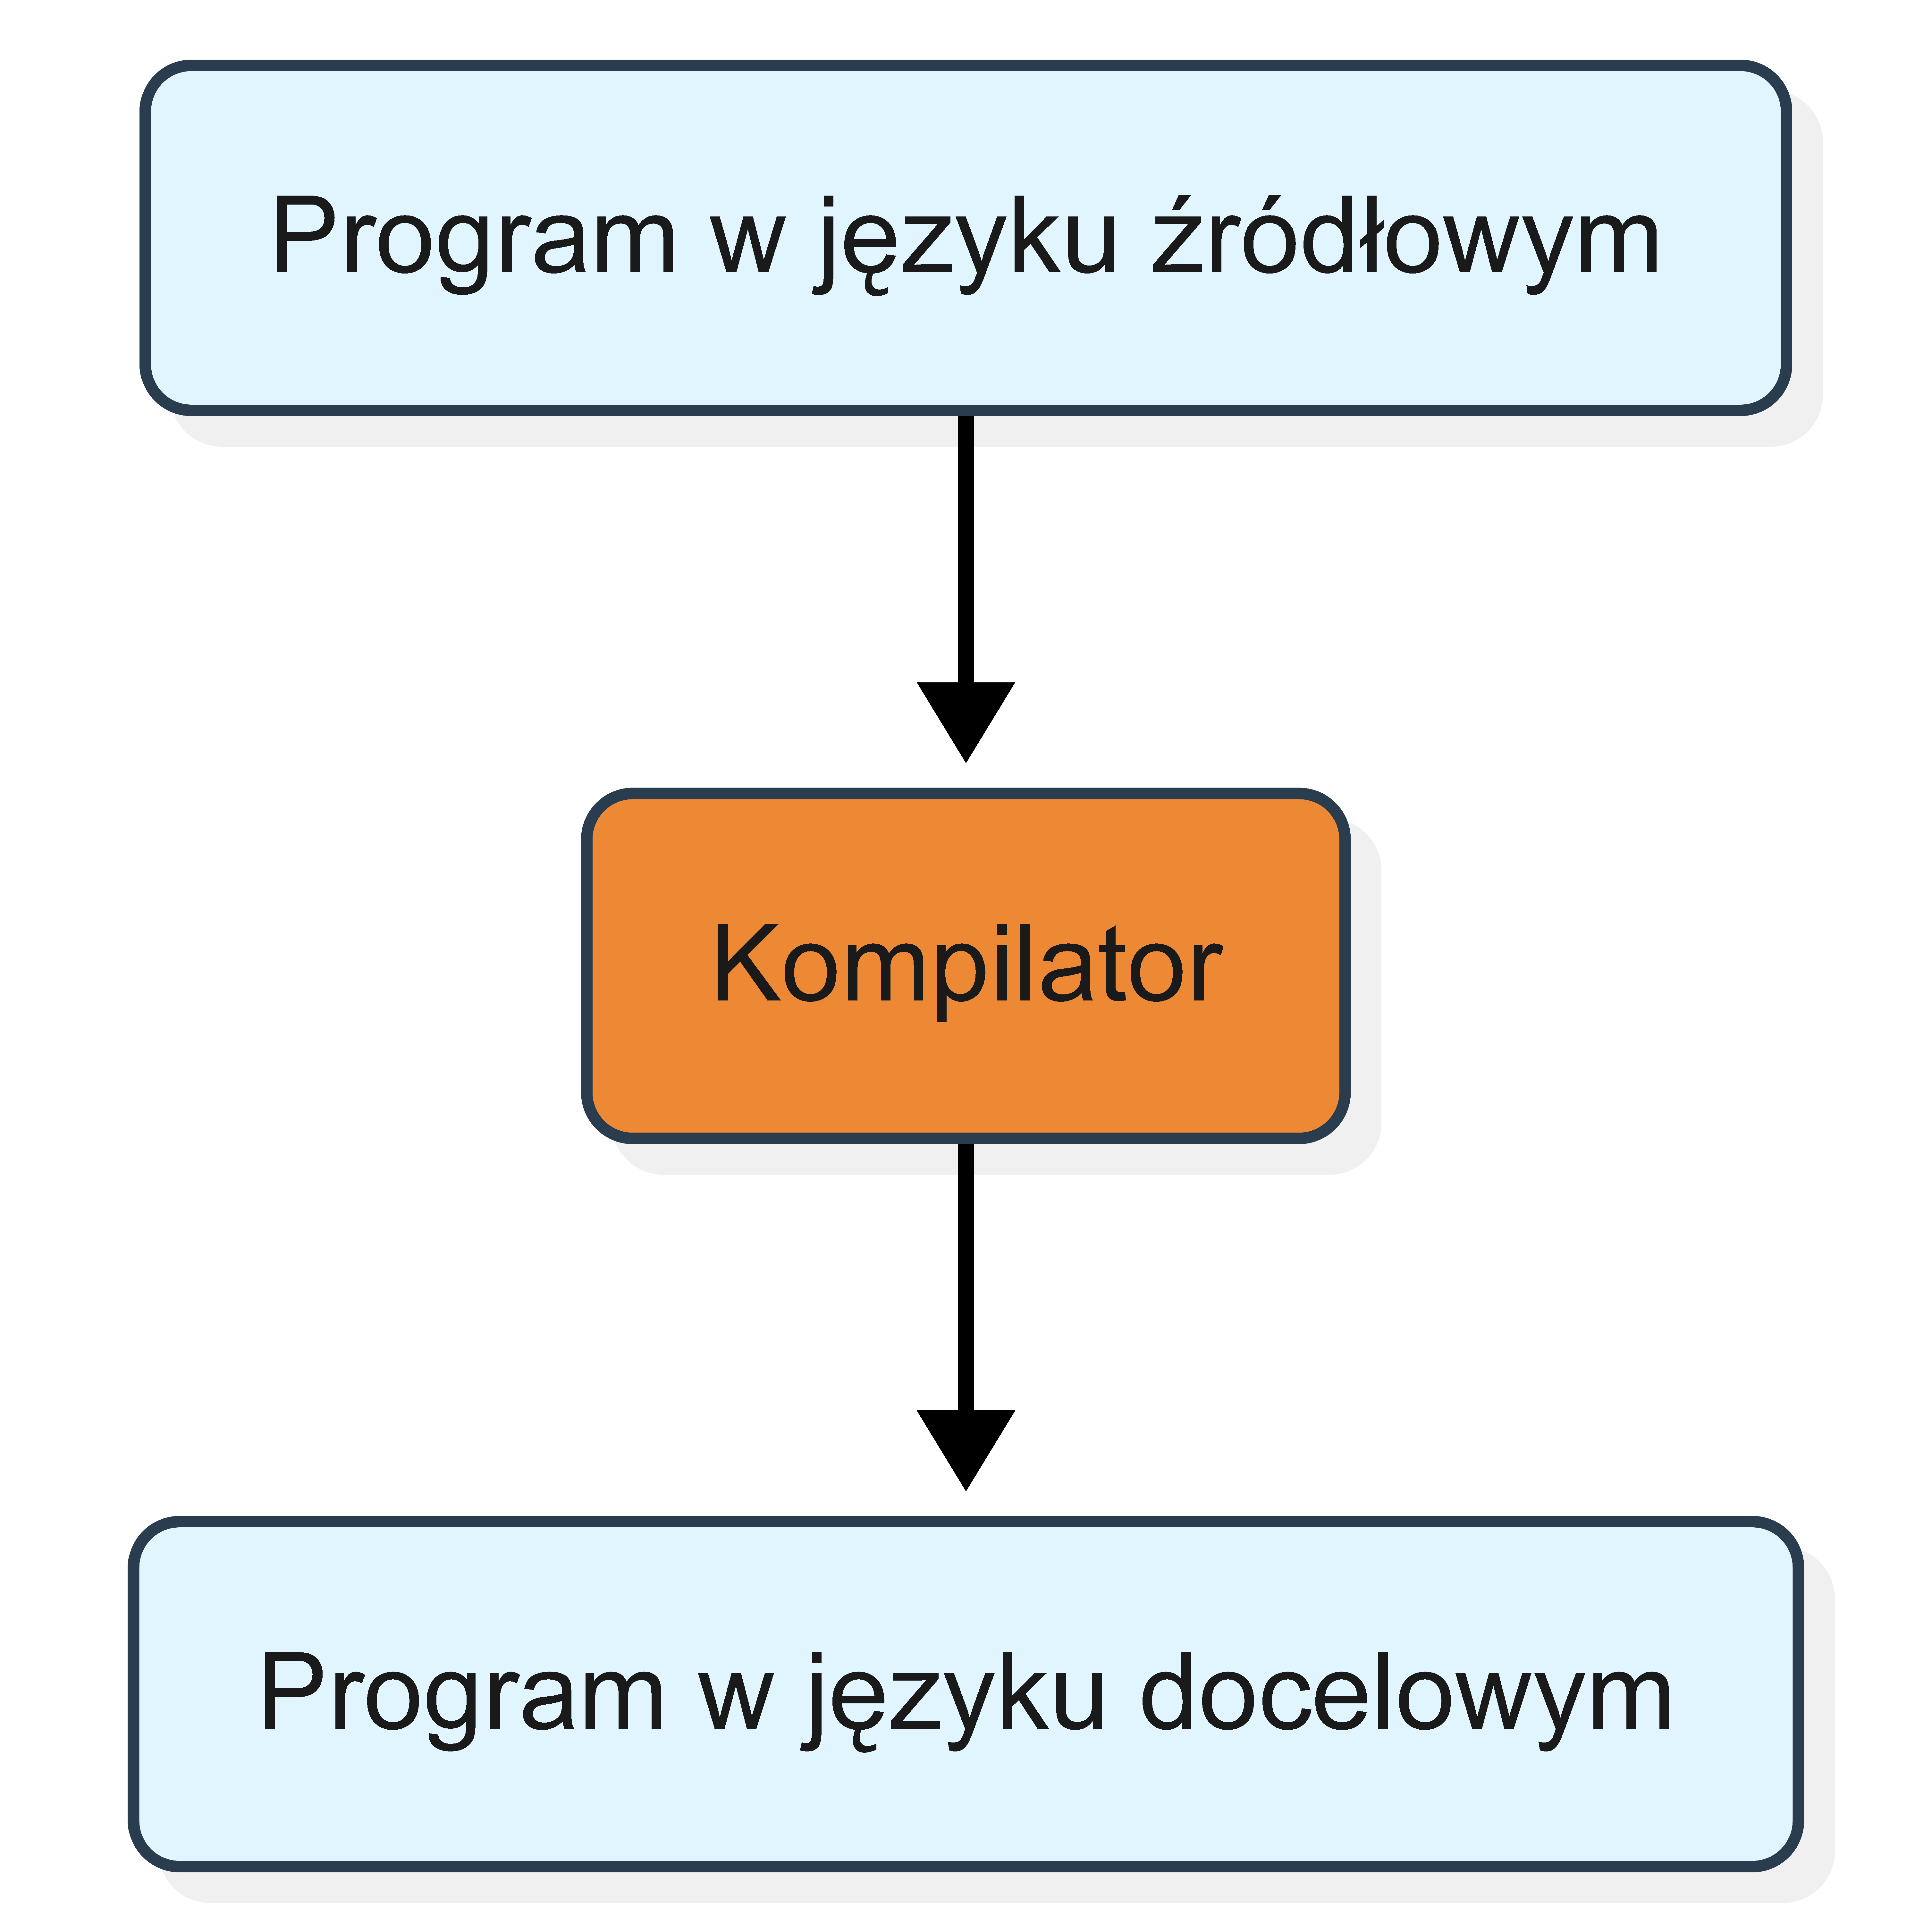
\includegraphics[width=0.6\textwidth]{img/Rysunek3.pdf}
    \caption{Model "czarnej skrzynki"~kompilatora}
    \label{fig:rysunek3}
\end{figure}

W systemach wbudowanych takie uproszczone podejście jest jednak często niewystarczające, ponieważ w takich zastosowaniach powszechnym zjawiskiem są silnie ograniczone zasoby sprzętowe, a nierzadko również ścisły rygor czasowy. Z tego względu programy tworzone przez inżyniera muszą być nie tylko poprawne pod kątem logicznym, ale również niezwykle rozsądnie gospodarować dostępnymi zasobami. Aby świadomie polepszać osiągi i kontrolować ten proces, konieczne jest porzucenie modelu czarnej skrzynki i zejście kilka poziomów abstrakcji niżej – począwszy od zrozumienia, jaki zestaw narzędzi jest w ogóle potrzebny do przetworzenia języka. 

Na potrzeby niniejszej pracy zostanie przytoczony sposób postępowania opisany w książce \cite{Kompilatory_Aho}, przedstawiony na schemacie \cref{fig:rysunek2}. Należy zaznaczyć, że zaprezentowany na rysunku pakiet oprogramowania, powszechnie określany jest przez użytkowników mianem kompilatora, choć w rzeczywistości zawiera w sobie zestaw wielu współpracujących programów komputerowych, w tym ten właściwy kompilator.
\begin{figure}[h]
    \centering
    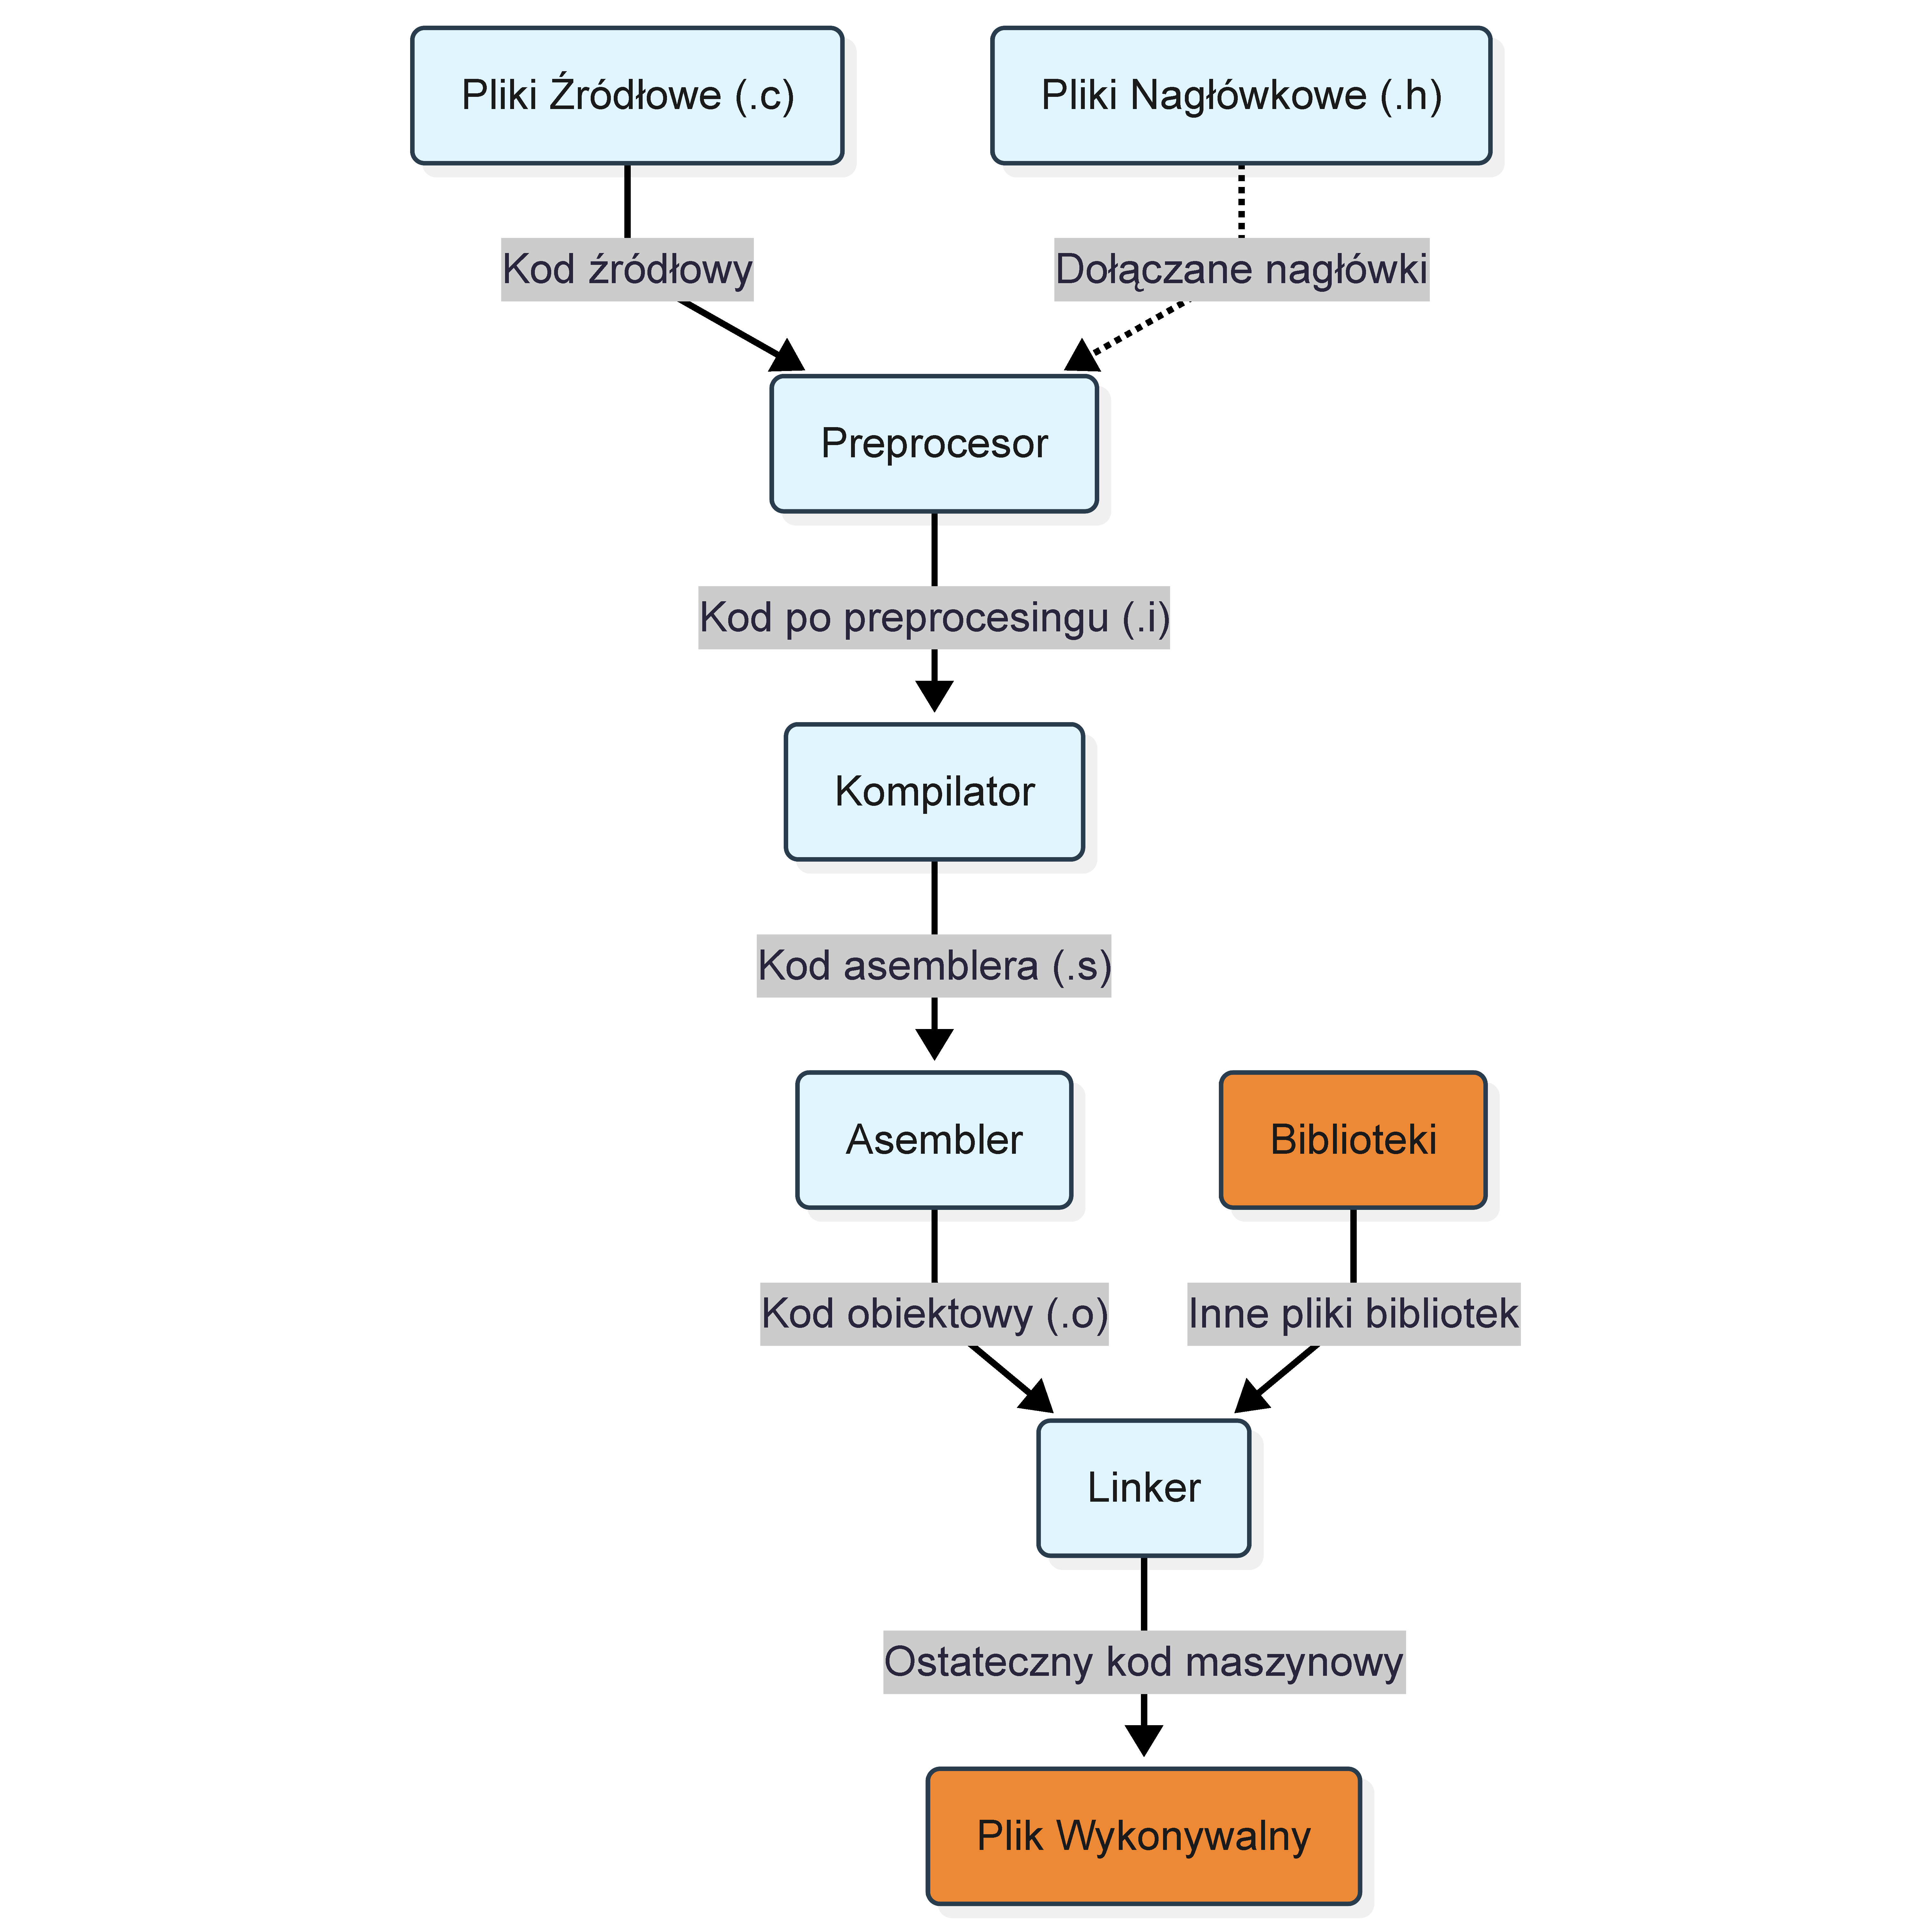
\includegraphics[width=0.8\textwidth]{img/Rysunek2.pdf}
    \caption{Klasyczny przebieg systemu przetwarzania języka programowania  \cite{Kompilatory_Aho}}
    \label{fig:rysunek2}
\end{figure}
Jak się okazuje, do utworzenia wykonywalnego programu docelowego wymagane jest najczęściej użycie kilku dodatkowych narzędzi, ułożonych w taki sposób, że wynik przetwarzania jednego jest wejściem dla kolejnego.
W klasycznym podejściu proces tworzenia pliku wykonywalnego składa się z następujących faz \cite{CinNutshell}:

\textbf{Preprocesor} odpowiada za przygotowanie kodu źródłowego przed jego właściwą analizą. Jego początkowym zadaniem jest zebranie programu, który nierzadko bywa podzielony na oddzielne moduły plikowe. Następnie program ten wykonuje odpowiednie dyrektywy oraz rozwija zdefiniowane przez programistę skróty (makra) do postaci pełnoprawnych instrukcji języka źródłowego.

\textbf{Kompilator} przyjmuje zmodyfikowany przez preprocesor kod i dokonuje jego tłumaczenia. Zazwyczaj wynikiem jego pracy nie jest bezpośredni kod maszynowy, lecz program zapisany w języku asemblera, powiązanym z docelową architekturą, na której uruchamiany ma zostać przygotowany program. Generowanie na tym etapie kodu asemblerowego wynika z faktu, iż jako język czytelny dla człowieka jest on znacznie łatwiejszy do wyprodukowania oraz ewentualnego debugowania.

\textbf{Asembler} zajmuje się przetworzeniem kodu asemblerowego na postać zrozumiałą dla maszyny. Wynikiem jego działania jest relokowalny kod maszynowy, zapisany w postaci tak zwanych plików obiektowych. Dodatkowo na tym etapie dla każdego z plików generowana jest tablica symboli, opisująca obiekty posiadające powiązania zewnętrzne \cite{CinNutshell}.

\textbf{Linker} łączy wygenerowane pliki obiektowe oraz niezbędne biblioteki w jeden spójny plik wykonywalny. Jego kluczowym zadaniem jest rozwiązanie adresów pamięci dla odwołań zewnętrznych pomiędzy poszczególnymi modułami programu, do czego wykorzystuje wspomniane wcześniej tablice symboli. W procesie tym linker dołącza również kod niezbędnych funkcji pochodzących ze standardowych lub zewnętrznych bibliotek \cite{CinNutshell}.

\subsection{Wewnętrzna struktura kompilatora}\label{subsection:WewStrukturaKompilatora}
%ta sekcja jest do poprawy, mamy 2 ksiazki compilter i dragon book z ktorych mozna sobie pokorzystac. 
Kompilator wewnętrznie dzieli się na dwie części: analizę (front end), która rozkłada program źródłowy na składowe elementy i na ich podstawie buduje reprezentację pośrednią oraz tablicę symboli, oraz syntezę (back end), która na tej podstawie konstruuje program docelowy \cite{Kompilatory_Aho}.

Proces ten przebiega jako sekwencja faz, z których każda przekształca jedną reprezentację programu w inną, a tablica symboli jest wykorzystywana przez wszystkie z nich \cite{Kompilatory_Aho}:

\begin{itemize}
    \item \textbf{Analiza leksykalna} - grupuje znaki programu źródłowego w leksemy i zamienia je na tokeny.
    \item \textbf{Analiza składniowa} - na podstawie tokenów buduje drzewo składniowe odzwierciedlające strukturę gramatyczną programu.
    \item \textbf{Analiza semantyczna} - sprawdza zgodność programu z definicją języka, w tym poprawność typów.
    \item \textbf{Generowanie kodu pośredniego} - tworzy niskopoziomową reprezentację programu, np. w postaci kodu trójadresowego.
    \item \textbf{Optymalizacja kodu} - opcjonalnie usprawnia kod pośredni, tak aby wynikowy kod docelowy był lepszy (np.\ szybszy lub mniejszy).
    \item \textbf{Generowanie kodu} - tłumaczy reprezentację pośrednią na kod maszyny docelowej, przydzielając m.in.\ rejestry zmiennym.
\end{itemize}

W praktycznych implementacjach kilka faz bywa łączonych w jeden przebieg (ang. \textit{pass}) \cite{Kompilatory_Aho}.


\section{Przegląd najpopularniejszych kompilatorów języka C}

Na rynku dostępnych jest wiele implementacji kompilatorów języka C, zarówno komercyjnych, jak i rozwijanych w modelu otwartoźródłowym. W praktyce jednak w środowisku systemów opartych na jądrze Linux najczęściej spotyka się dwa rozwiązania: \textbf{GNU Compiler Collection (GCC)}, powstały w ramach projektu GNU \cite{StallmanGNU}, oraz \textbf{Clang}, będący częścią projektu \textbf{LLVM}.\
Samo jądro systemu Linux przez długi okres było kompilowane było wyłącznie narzędziami GNU, jednak w ostanim czasie Clang i LLVM stały się dla nich dostepną alternatywą -- kompilowane z ich wykorzstaniem jądra systemu Linux wykorzystują między innymi systemy Android czy ChromeOS \cite{KernelLLVM}.

Warto zaznaczyć, że również w systemach wbudowanych, niewykorzystujących systemów operacyjnych, narzędzia GNU czy Clang wraz z LLVM są często spotykane. Oferują one wsparcie dla wielu architektur procesorów, pozwalając na uruchomienie kompilatora na sprzęcie o jednej architekturze (nazywanej również terminem \textbf{maszyny hosta}) w celu wygenerowania kodu maszynowego przeznaczonego dla zupełnie innej, docelowej architektury (nazywanej \textbf{maszyną targetu}). Proces ten określany jest mianem \textbf{kompilacji skrośnej} (ang. \textit{cross-compilation}). Obydwa wspomniane kompilatory posiadają zestaw narzędzi przeznaczonych do różnych architektur spotykanych w systemach wbudowanych, takich jak \textbf{ARM, RISC-V, AVR}.
\subsection{Kompilator GCC}

\textbf{GCC} powstał jako część projektu GNU \cite{StallmanGNU} i jest tradycyjnym, domyślnym kompilatorem większości dystrybucji systemu Linux \cite{LinuxKernelDevelopment}. Jego architektura rozwiązań bazuje na klasycznym modelu kompilatora, który opisuje \cref{subsection:WewStrukturaKompilatora}. GCC dzieli proces tłumaczenia na część analizującą (front end) i część generującą kod wynikowy (back end). Część środkowa, odpowiedzialna za optymalizacje, przekształca program w dwóch własnych, uproszczonych reprezentacjach -- GENERIC oraz GIMPLE -- na których wykonywane są kolejne przekształcenia mające na celu poprawnienie kodu \cite{novillo2006gcc}. 
\subsection{Kompilator Clang}

\textbf{Clang} pełni rolę części analizującej (front end) dla  części syntezy obsługiwanej przez \textbf{LLVM}. LLVM zapewnia zestawu narzędzi kompilatorowych, zaprojektowanego tak, aby umożliwić analizę i poprawianie kodu na każdym etapie jego translacji i uruchomienia \cite{lattner2004llvm}. Podobnie jak GCC, LLVM przekształca program do własnej, uproszczonej reprezentacji pośredniej, jednak w odróżnieniu od GCC reprezentacja ta została zaprojektowana w taki sposób, aby nie musięć zależeć od konkretnego języka programowania \cite{lattner2004llvm}. Dzięki takiej budowie LLVM można podzielić na trzy niezależne części: część analizującą (Clang), wspólną dla wszystkich architektur warstwę optymalizacji oraz część generującą kod maszynowy dla konkretnego procesora. Kod projektu LLVM, w tym Clang, jest udostępniany na licencji Apache License \cite{LLVMDevPolicy}.

Oba kompilatory, mimo różnic w budowie wewnętrznej, są ze sobą często porównywane w literaturze pod kątem jakości i wydajności generowanego kodu, w tym w zastosowaniach wbudowanych systemów wbudowanych \cite{poorhosseini2020compiler}.Oba rozwiązania dysponują bowiem wbudowanymi mechanizmami zaawansowanej optymalizacji kodu, o których traktuje \cref{section:TechnikiOptymalizacji}. Proces ten może być kontrolowany przez inżyniera oprogramowania poprzez stosowanie \textbf{flag kompilacji}, czyli poleceń określających pożądany stopień i cel optymalizacji programu docelowego. \cref{section:flagiKompilatora} przybliża dostępne flagi dla obywdu opisywanych kompilatorów.
\section{Zaawansowane techniki optymalizacji kodu}\label{section:TechnikiOptymalizacji}
\section{Flagi kompilacji dostępne w kompilatorach Clang i Gcc}\label{section:flagiKompilatora}

\begin{table}[htbp]
    \centering
    \caption{Poziomy optymalizacji w kompilatorach GCC i Clang, na podstawie oficjalnych dokumentacji\cite{gcc_optlevels,clang_cmdguide}}
    \label{tab:poziomy_optymalizacji}
    \begin{tabularx}{\textwidth}{@{} l X X @{}}
        \toprule
        \textbf{Flaga} & \textbf{GCC} & \textbf{Clang} \\
        \midrule

        \texttt{-O0} &
            Brak optymalizacji (ustawienie domyślne). Generuje nieoptymalny kod, lecz zapewnia najkrótszy czas kompilacji i najlepsze warunki do debugowania. &
            Oznacza brak optymalizacji -- najszybsza kompilacja i najlepiej debugowalny kod wynikowy. \\
        \addlinespace

        \texttt{-O1} &
            Umiarkowana optymalizacja (odpowiednik samego \texttt{-O}). Rozsądnie optymalizuje kod bez istotnego wydłużenia czasu kompilacji, choć część zmiennych może być niedostępna w debuggerze. &
            Poziom pośredni między \texttt{-O0} a \texttt{-O2}. \\
        \addlinespace

        \texttt{-O2} &
            Rozszerzona optymalizacja generująca silnie zoptymalizowany kod kosztem wydłużonego czasu kompilacji; istotnie utrudnia pracę z debuggerem. &
            Umiarkowany poziom optymalizacji włączający większość dostępnych optymalizacji. \\
        \addlinespace

        \texttt{-O3} &
            Pełna optymalizacja obejmująca bardziej zaawansowane przekształcenia, zwłaszcza pętli, potencjalnie kosztem większego rozmiaru kodu wynikowego. Praca z debuggerem jest w praktyce bardzo utrudniona. &
            Odpowiednik \texttt{-O2} rozszerzony o optymalizacje wymagające dłuższego czasu kompilacji lub zwiększające rozmiar kodu, w celu poprawy szybkości wykonania. \\
        \addlinespace

        \texttt{-Os} &
            Optymalizacja pod kątem rozmiaru kodu i danych zamiast szybkości; bazuje na \texttt{-O2} z wyłączeniem przekształceń zwiększających rozmiar binarki oraz dodatkowymi optymalizacjami redukującymi rozmiar. &
            Odpowiednik \texttt{-O2} z dodatkowymi optymalizacjami zmniejszającymi rozmiar kodu wynikowego. \\
        \addlinespace

        \texttt{-Oz} &
            Agresywna optymalizacja rozmiaru kodu i danych; może zwiększyć liczbę wykonywanych instrukcji, jeśli wymagają one mniejszej liczby bajtów do zakodowania. &
            Odpowiednik \texttt{-Os}, lecz z jeszcze dalszą redukcją rozmiaru kodu wynikowego. \\
        \addlinespace

        \texttt{-Og} &
            Optymalizacja zorientowana na komfort debugowania zamiast szybkości; bazuje na \texttt{-O1}, dążąc do wyeliminowania negatywnego wpływu optymalizacji na proces debugowania. &
            Zbliżony do \texttt{-O1}, lecz z nieco ograniczoną optymalizacją i lepszą widocznością zmiennych; dodatkowo ustawia flagę \texttt{-fextend-variable-liveness}, poprawiającą dostępność zmiennych podczas debugowania. \\
        \addlinespace

        \texttt{-Ofast} &
            Poziom nieuwzględniony w cytowanym dokumencie GNAT jako osobna flaga GCC (w praktyce GCC obsługuje \texttt{-Ofast} analogicznie do Clang -- zob.\ kolumna obok). &
            Włącza wszystkie optymalizacje z \texttt{-O3} wraz z dodatkowymi agresywnymi optymalizacjami mogącymi naruszać ścisłą zgodność ze standardem języka (m.in.\ \texttt{-ffast-math}). Flaga oznaczona jako przestarzała od Clang 19. \\

        \bottomrule
    \end{tabularx}

    \vspace{0.5em}
\end{table}



